\frameT{Preferences Are Ubiquitous}{
	\begin{figure}[ht!]
	  \centering
	    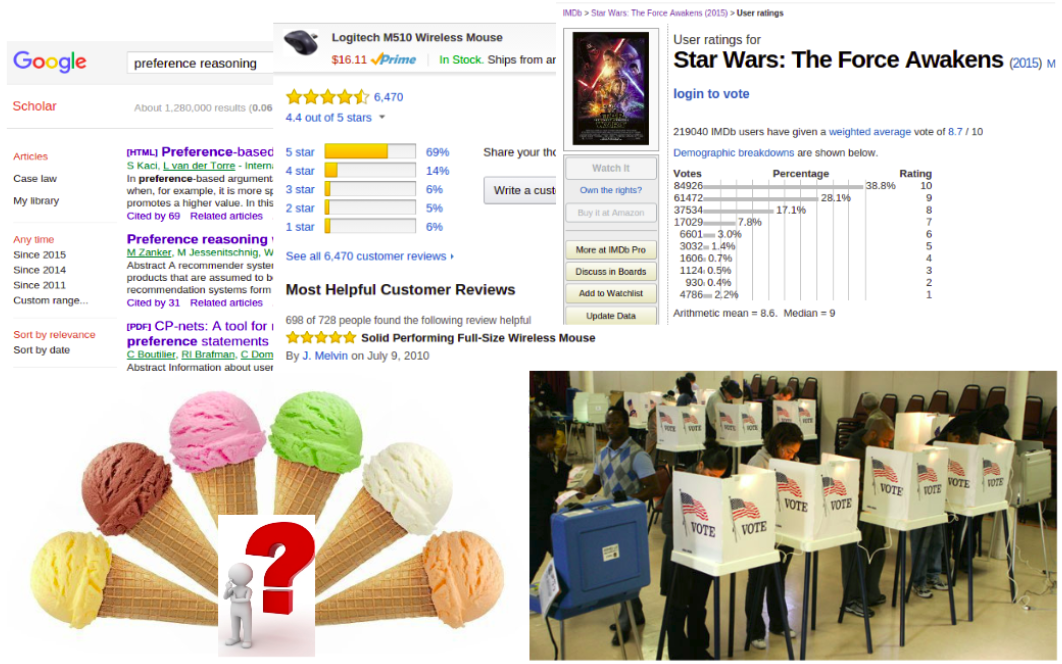
\includegraphics[width=0.8\textwidth]{figs/PrefApplications/pref_applications.png}
	  \caption{Preferences of different forms}
	\end{figure}
}

\frameT{Describing Preferences}{
	\begin{figure}[ht!]
	  \centering
	    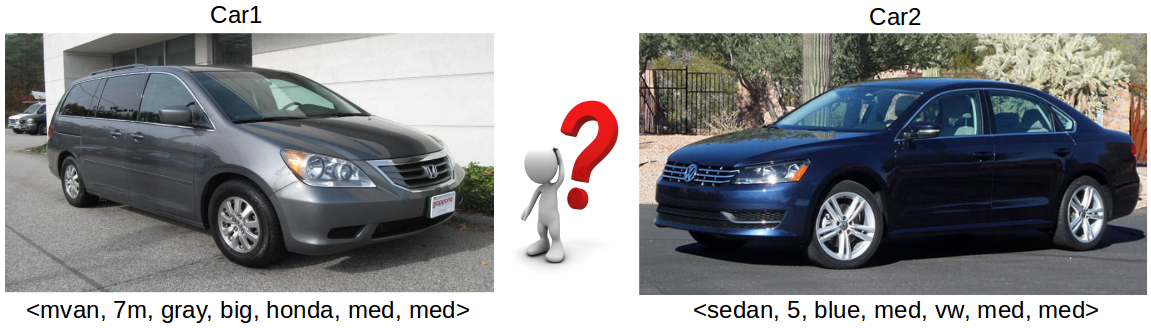
\includegraphics[width=0.95\textwidth]{figs/Cars/individual.png}
	  \caption{How to express preferences?}
	\end{figure}

	\vspace{-0.7cm}

	\begin{enumerate}
		\item How will I rate cars?
		\begin{itemize}
			\item For BodyType, I will assign 7 points to minivans, 5 to sedans, ...
			\item For Color, I will assign 8 points to blue, 4 to gray, ...
		\end{itemize}
		\item What are the desired properties I see in cars?
		\begin{itemize}
			\item I prefer minivans to sedans, ...
			\item If minivan, I prefer gray to blue; if sedan, I prefer blue to gray; ...
		\end{itemize}
	\end{enumerate}
}

\frameT{Describing Preferences}{
	\begin{figure}[ht!]
	  \centering
	    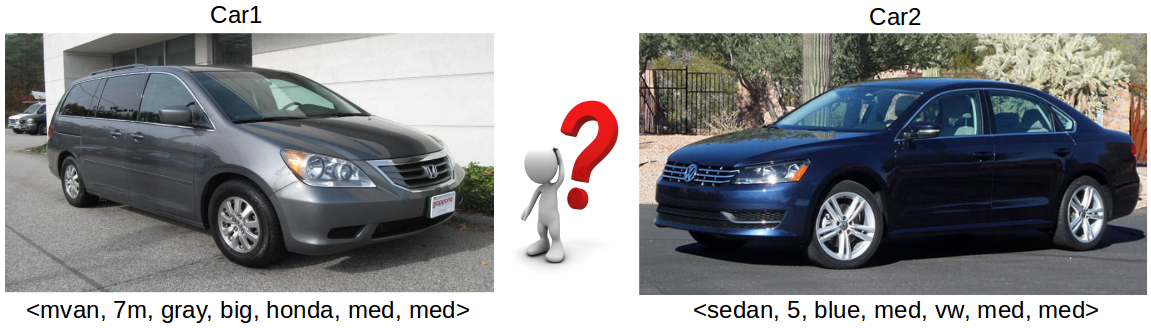
\includegraphics[width=0.95\textwidth]{figs/Cars/individual.png}
	  \caption{How to express preferences?}
	\end{figure}

	\vspace{-0.7cm}

	\begin{enumerate}
		\item How will I rate cars? (\tbf{Quantitative})
		\begin{itemize}
			\item For BodyType, I will assign 7 points to minivans, 5 to sedans, ...
			\item For Color, I will assign 8 points to blue, 4 to gray, ...
		\end{itemize}
		\item What are the desired properties I see in cars? (\tbf{Qualitative})
		\begin{itemize}
			\item I prefer minivans to sedans, ...
			\item If minivan, I prefer gray to blue; if sedan, I prefer blue to gray; ...
		\end{itemize}
	\end{enumerate}
}
